\documentclass[a5paper,12pt]{article}
\usepackage{../../style}


\newcommand{\montitre}{POO }


\begin{document}

\fiche{Introduction}
\titre{Principes de la POO} : 
\begin{enumerate}
	\item Objet
	\item Méthode
	\item Classe
	\item Hiérarchie de classes
\end{enumerate}

\titre{Exemple : définition de la structure conditionnelle en smallTalk}\\
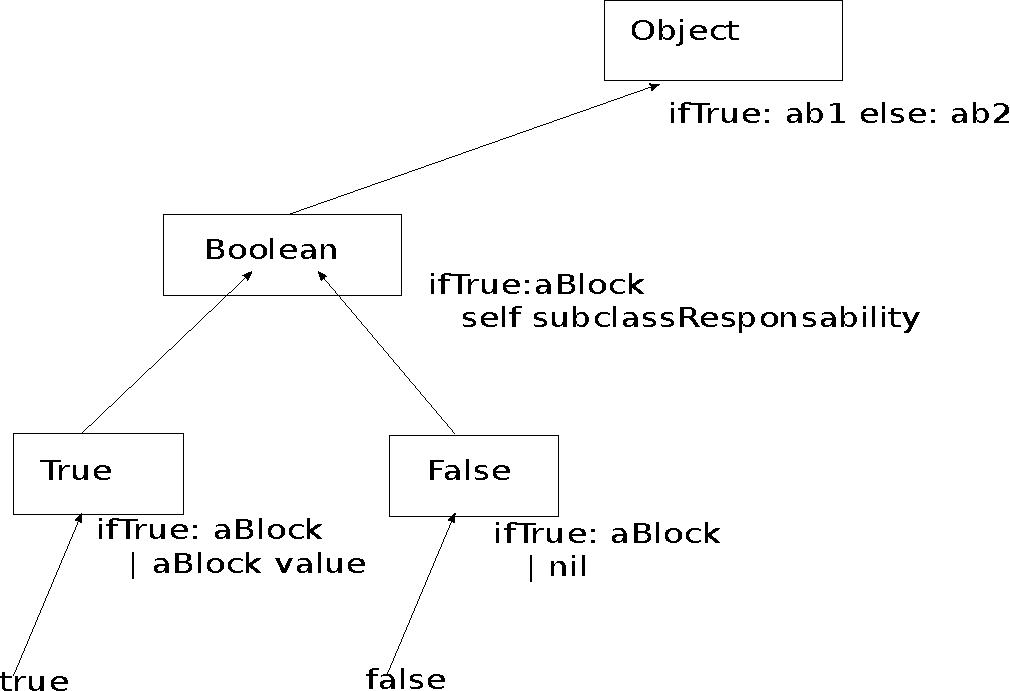
\includegraphics[width=180px]{Images/fig1.pdf}

\titre{Plan de cours}
\begin{enumerate}
	\item Introduction
	\item Concepts de base (objet, classe, envoi de message, hiérarchie)
	\item Illustrations et exemples (Java, Simula, SmallTalk
	\item Etude comparative de LO
	\item TP (Java, Eclipse)
\end{enumerate}

\titre{Histoire d'Ada}
Le département de la défense américain (Dod) est : 
\begin{itemize}
	\item Plus gros consommateur de logiciels
	\item 1968 - 73 : Le coût des SI augmente et le coût du matériel chute
	\item 73 : 7,5 milliards de dollars pour les Si
	\item 75 : 450 langages différents
	\item Réutilisabilité et partage de code inexistants
	\item 1983 : naissance d'Ada en réponse à la crise du logiciel et pour résoudre les pbs liés au dev de gros logiciels
	\item non issu d'un projet académique ou de recherche interne
\end{itemize}
Idée : Un seul langage incorporant tous les bons concepts de GL.\\

\titre{Paradigmes de programmation}
\begin{itemize}
	\item impérative
	\item fonctionnelle
	\item logique
	\item objet
	\item par contraintes
\end{itemize}

\newpage

\titre{Les domaines révolutionnés par la POO}
\begin{itemize}
	\item Génie logiciel (analyse, conception, programmation)
	\item Bases de données
	\item Intelligence artificielle (représentation des connaissances, programmation par agents)
\end{itemize}

\titre{Quel objet ?}
\begin{itemize}
	\item Des problématiques différentes $\rightarrow$ Des approches objet différentes
	\item Une préoccupation commune (approche modulaire de la complexité)
\end{itemize}
Pour distinguer les approches différentes, on change le voc :
\begin{itemize}
	\item Génie Logiciel : Objet
	\item IA : Schéma
	\item Ingénierie collaborative : Agent
	\item Bases de données : RDF
\end{itemize}

\titre{Quels languages :}
\begin{itemize}
	\item Java sous éclipse principalement
	\item Simula
	\item SmallTalk
\end{itemize}


\fiche{Concepts de base}
\titre{Programmation impérative :} C'est un paradigme de programmation qui décrit les opérations en termes d'états du programme et de séquences d'instructions exécutées par l'ordinateur pour modifier l'état du programme. \\ Les paramètres sont passés par valeur. \\
Elle repose sur deux principes :
\begin{itemize}
	\item Séparation des programmes et des données.
	\item Priorité donnée aux traitements (alors qu'en fait ce sont les structures de données qui sont les plus stables).
\end{itemize}

On aimerait donc pouvoir manipuler des objets définis par leurs caractéristiques externes (protocoles) indépendamment de toute représentation interne $\rightarrow$ Ada (reste impératif car il permet la POO mais ne fanchit pas le pas de le rendre obligatoire). \\

\titre{Remarque :} 
\begin{itemize}
	\item Révolution Algol/Ada : associer des données à des programmes (variables locales, paramètres)
	\item Révolution Objet : associer des programmes à des données
\end{itemize}



\fiche{Notion de programmation objet}
\titre{Définition :} Manipuler des objets définis par leurs caractéristiques externes (protocoles) indépendamment de toute représentation interne. \\

\titre{Deux manières de faire :}
\begin{itemize}
	\item Langage impératif + Constructions syntaxiques 
		\begin{itemize}
			\item regrouper les données et les programmes
			\item protéger (cacher, exporter)
			\item Séparer spécification et implémentation
			\item $\rightarrow$ on compte sur le bon sens du programmeur
			\item exemples : ADA, Pascal
		\end{itemize}
	\item Langage objet
		\begin{itemize}
			\item Définir de nouveaux types, et les manipuler (c'est la manipulation qui fait la différence avec les langages impératifs)
			\item Différence entre les types prédéfinis et types utilisateurs (ne devrait pas exister dans un langage purement objet)
			\item exemples : Simula67, SmallTalk80, Common Lisp objet, Eiffel, C++, Java, Objective C, Ruby, Python, C\#, Groovy, Lisaac
		\end{itemize}
\end{itemize}

\titre{Type abstrait :}
\begin{itemize}
	\item Données
	\item Opérateurs
	\item Propriétés
\end{itemize}

\titre{Caractéristiques}
\begin{itemize}
	\item Modularité
	\item Sécurité
	\item Spécification
	\item Réutilisabilité
\end{itemize}

\titre{Exemple :} Pile d'entiers
\begin{itemize}
	\item Pile, Entier, Booléen
	\item 
		\begin{itemize}
			\item pile\_vide : Pile $\rightarrow$ Booléen
			\item empiler : Pile $\times$ Entier $\rightarrow$ Pile
			\item depiler : Pile $\rightarrow$ Piles $\times$ Entier
		\end{itemize}
	\item
		\begin{itemize}
			\item non(pile\_vide(empiler(p,e)))
			\item depiler(empiler(p,e)) = (p,e)
			\item non(pile\_vide(p)) $\impl$ empiler(depiler(p)) = p
		\end{itemize}
\end{itemize}

\titre{Approche descriptive}
\begin{itemize}
	\item La réalité est composée d'objets (perçu, concret, animé ou non, conçu, abstrait) $\rightarrow$ connaissance singulière
	\item Caractéristiques contingentes (peu varier) $\rightarrow$ attributs
	\item Caractéristiques essentielles (intrinsèque) $\rightarrow$ classes différentes
	\item Objet $\rightarrow$ Concept (abstraction de classes : fox $\rightarrow$ voiture $\rightarrow$ moyen de locomotion)
	\item Concept $\rightarrow$ Exemplification (spécialisation de classe : moyen de locomotion $\rightarrow$ voiture $\rightarrow$ fox
\end{itemize}

\titre{Approche service (fonctionnelle) :} Objet $\equiv$ Composant. L'accent est mis sur les caractéristiques externes, descriptives et comportementales de l'objet. \\ \\
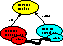
\includegraphics[width=150px]{Images/fig2.pdf} \hspace{1cm}

\includegraphics[width=150px]{Images/fig3.pdf} \\
\begin{itemize}
	\item Encapsulation des données, boite noire
	\item Un objet permet de regrouper en une seule entité et de façon indissociable données et procédures d'exploitation.
	\item Un objet est une instance de classe 
		\begin{itemize}
			\item ses données sont les variables d'instance, attributs variables, données membres. Les données sont accessibles uniquement à traver les procédures (programmation par état) $\rightarrow$ c'est rémanent (ie si l'objet se modifie lors d'une procédure, alors l'état initial n'est pas restauré). \\
			Remarque : En Java, l'unité d'encapsulation est la classe (les objets d'une même classe peuvent accéder aux champs privés des autres instances de la même classe). Ca devrait être l'objet.
			\item Les procédures sont les méthodes, attributs procédures, fonctions membres. Il y a des méthodes exportées (elles définissent l'interface) et des méthodes cachées (utiles uniquement à l'implémentation)
		\end{itemize}
\end{itemize}

\titre{Programmation par état :}
	\begin{itemize}
		\item On travaille par référence et non par valeur
		\item En java, les types primitifs passent par valeur
	\end{itemize}

\titre{Exemple :} Processus
\begin{itemize}
	\item Que \titre{fait} un processus ?
	\begin{itemize}	
		\item Suspendre
		\item Réveiller
		\item Priorité
	\end{itemize}
	\item Qu'\titre{est} un processus ? 
	\begin{itemize}
		\item Ressources
		\item Contexte
		\item Programme
	\end{itemize}
	\item $\rightarrow$ Ces deux points de vue peuvent être mixés par l'héritage multiple, mais nous en général on choisira une des deux approches et on s'y tiendra.
\end{itemize}


\fiche{Héritage multiple}
\titre{Exemple :} NoeudPersonne hérite de Noeud(méthodes de gestion d'un noeud), et de Personne(méthodes de gestion d'une personne. Si l'héritage multiple n'est pas géré, on peut hériter de Noeud uniquement avec une instance de Personne, ou utiliser un objet composite avec un attribut Noeud et un attribut Personne.\\

\titre{Problème :} Définir un sous-concept à partir de plusieurs sur-concepts a-t-il un sens ?


\fiche{Classes abstraites et terminales}
\titre{Règle :} Seules les classes terminales peuvent être instanciées. Toute classe possédant des spécialisations est une classe abstraite (ne peut être instanciée). Les extensions des classes terminales d'une classe générique constituent une partition de l'ensemble des instances relevant de la classe générique (classe de base, abstraite).


\end{document}
